
\noindent\textbf{Any}
\lstinputlisting[firstline=1,lastline=3]{../transformations/sequence/emftvm/TestAny.atl}
\begin{figure*}[h]
\centering	
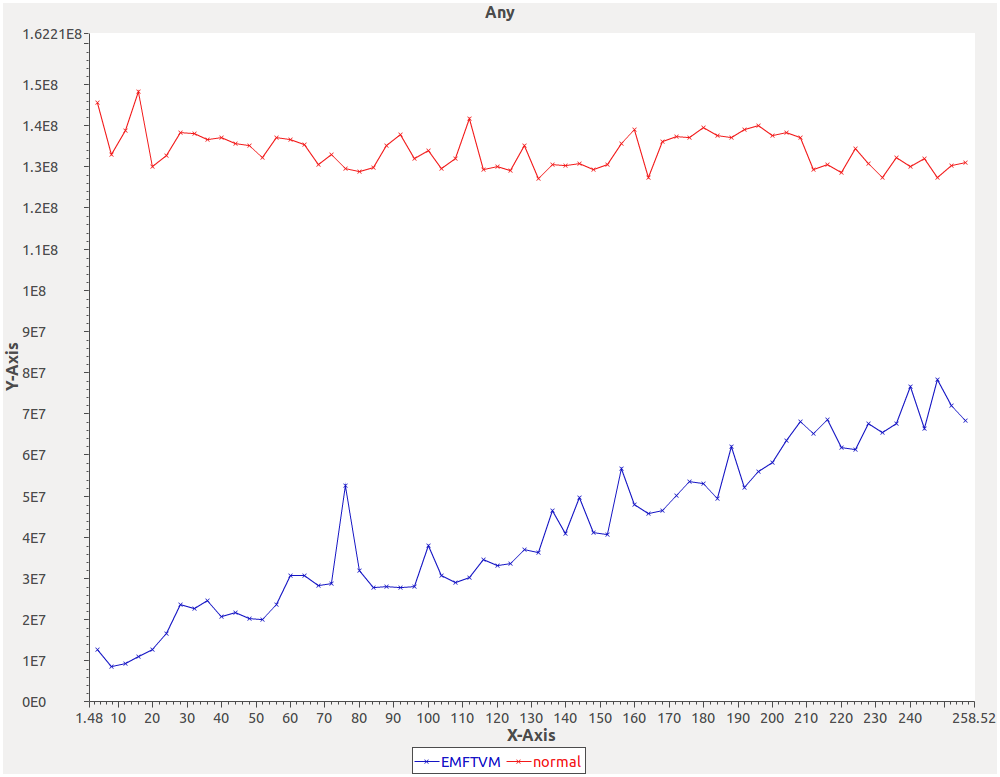
\includegraphics[width=\textwidth]{../graphs/sequence/Any}
\end{figure*}
\pagebreak

\noindent\textbf{Append}
\lstinputlisting[firstline=1,lastline=3]{../transformations/sequence/emftvm/TestAppend.atl}
\begin{figure*}[h]
\centering
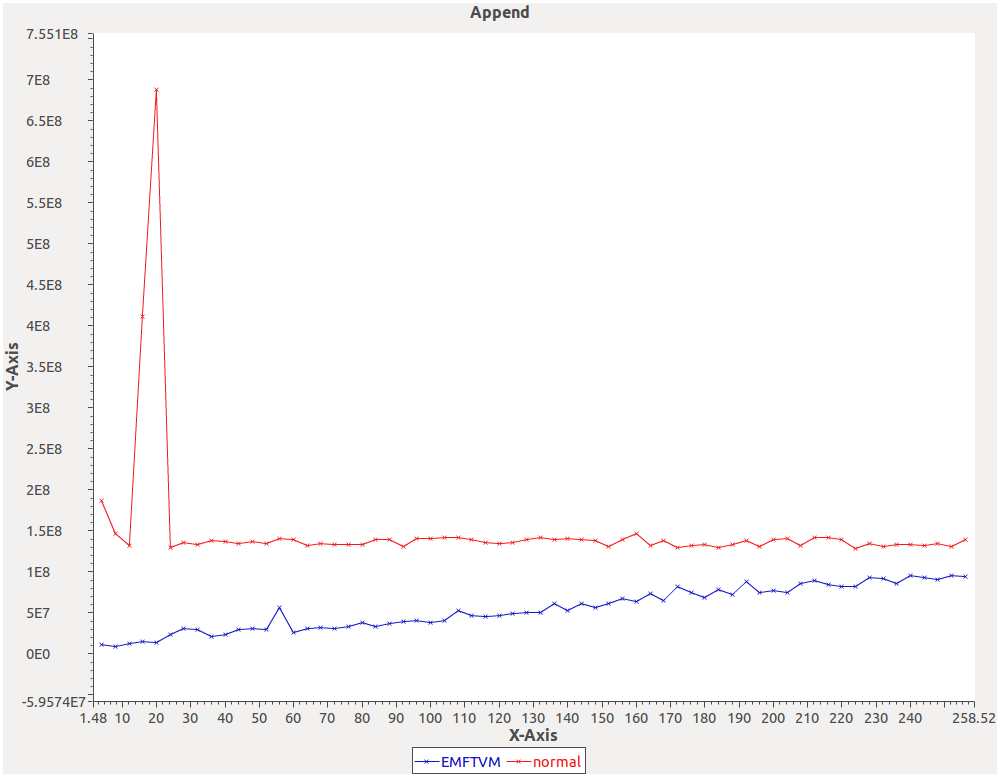
\includegraphics[width=\textwidth]{../graphs/sequence/Append}
\end{figure*}
\pagebreak

\noindent\textbf{At}
\lstinputlisting[firstline=1,lastline=3]{../transformations/sequence/emftvm/TestAt.atl}
\begin{figure*}[h]
\centering
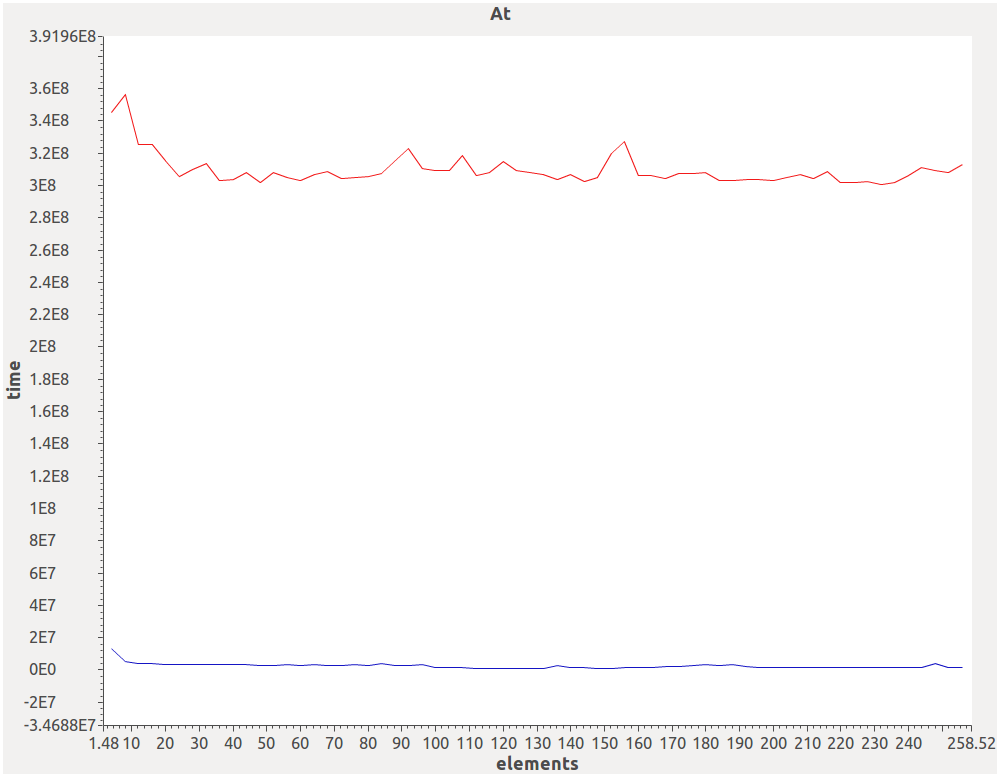
\includegraphics[width=\textwidth]{../graphs/sequence/At}
\end{figure*}
\pagebreak

\noindent\textbf{Collect}
\lstinputlisting[firstline=1,lastline=3]{../transformations/sequence/emftvm/TestCollect.atl}
\begin{figure*}[h]
\centering
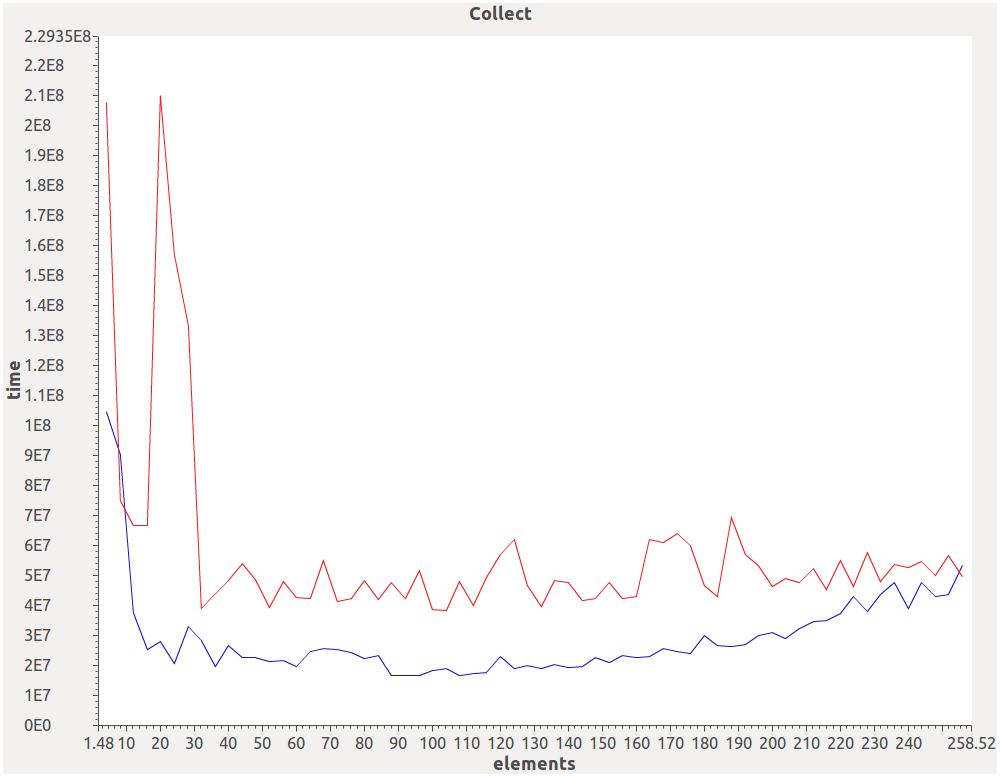
\includegraphics[width=\textwidth]{../graphs/sequence/Collect}
\end{figure*}
\pagebreak

\noindent\textbf{EQ}
\lstinputlisting[firstline=1,lastline=3]{../transformations/sequence/emftvm/TestEQ.atl}
\begin{figure*}[h]
\centering
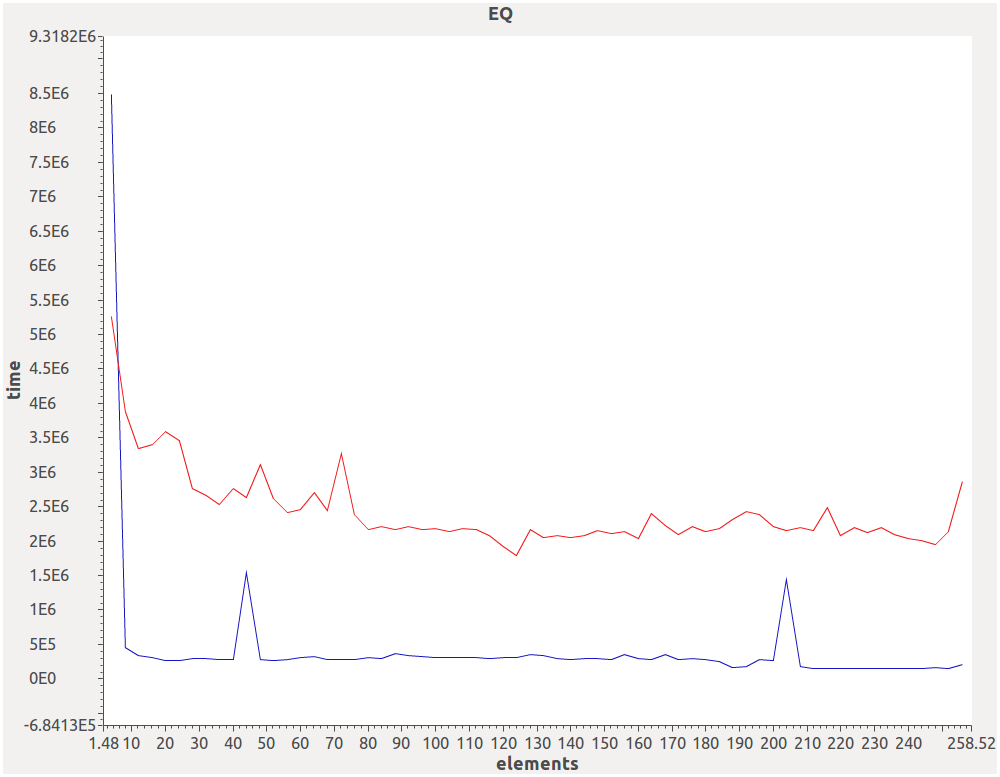
\includegraphics[width=\textwidth]{../graphs/sequence/EQ}
\end{figure*}
\pagebreak

\noindent\textbf{Excludes}
\lstinputlisting[firstline=1,lastline=3]{../transformations/sequence/emftvm/TestExcludes.atl}
\begin{figure*}[h]
\centering
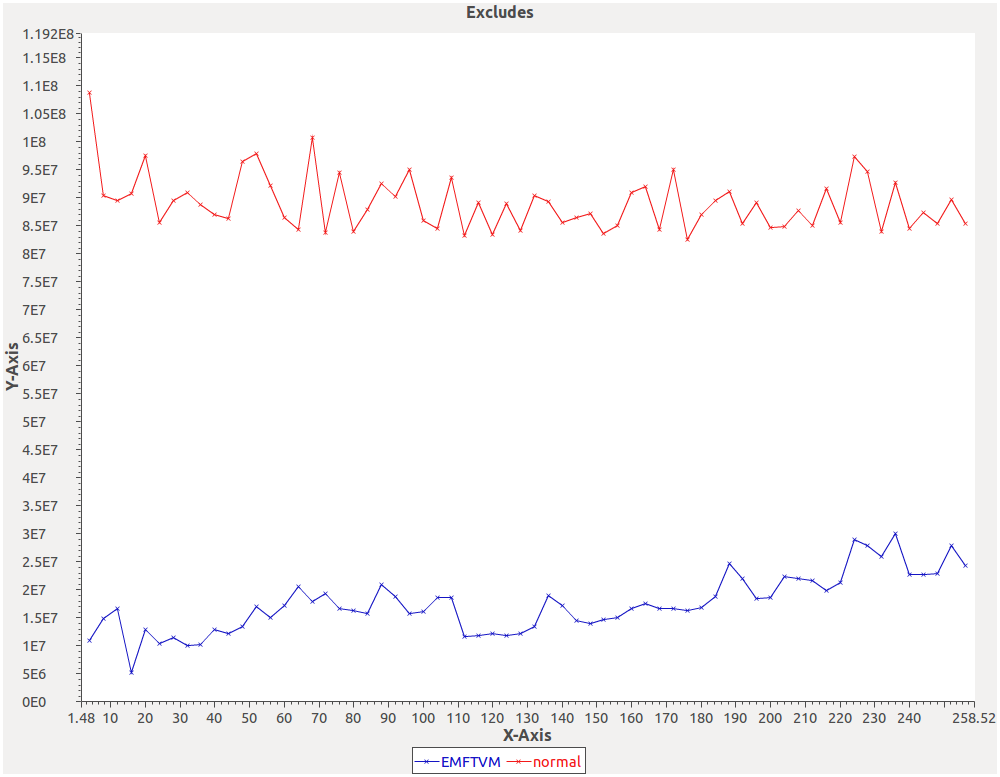
\includegraphics[width=\textwidth]{../graphs/sequence/Excludes}
\end{figure*}
\pagebreak

\noindent\textbf{ExcludesAll}
\lstinputlisting[firstline=1,lastline=3]{../transformations/sequence/emftvm/TestExcludesAll.atl}
\begin{figure*}[h]
\centering
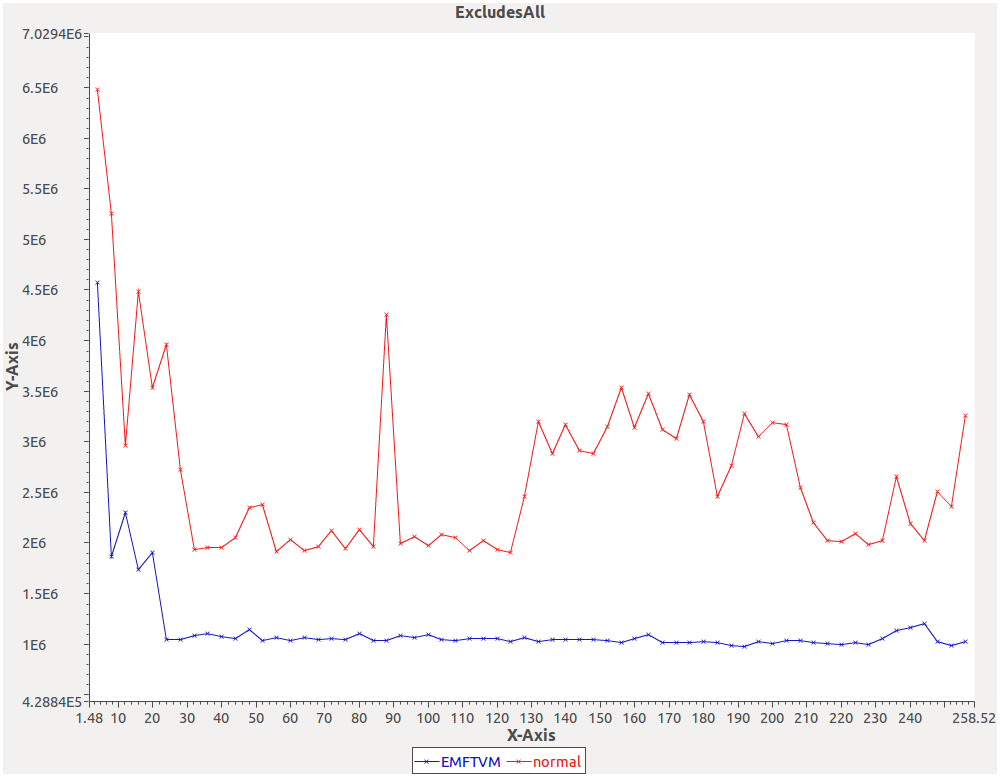
\includegraphics[width=\textwidth]{../graphs/sequence/ExcludesAll}
\end{figure*}
\pagebreak

\noindent\textbf{Excluding}
\lstinputlisting[firstline=1,lastline=3]{../transformations/sequence/emftvm/TestExcluding.atl}
\begin{figure*}[h]
\centering
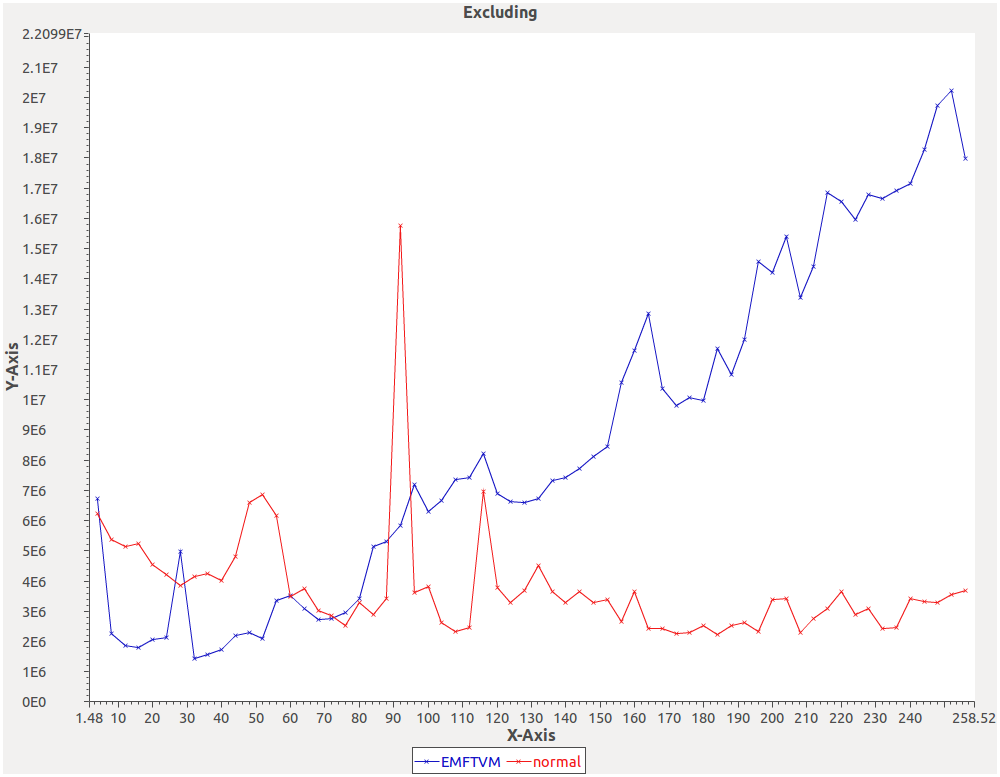
\includegraphics[width=\textwidth]{../graphs/sequence/Excluding}
\end{figure*}
\pagebreak

\noindent\textbf{Exists}
\lstinputlisting[firstline=1,lastline=3]{../transformations/sequence/emftvm/TestExists.atl}
\begin{figure*}[h]
\centering
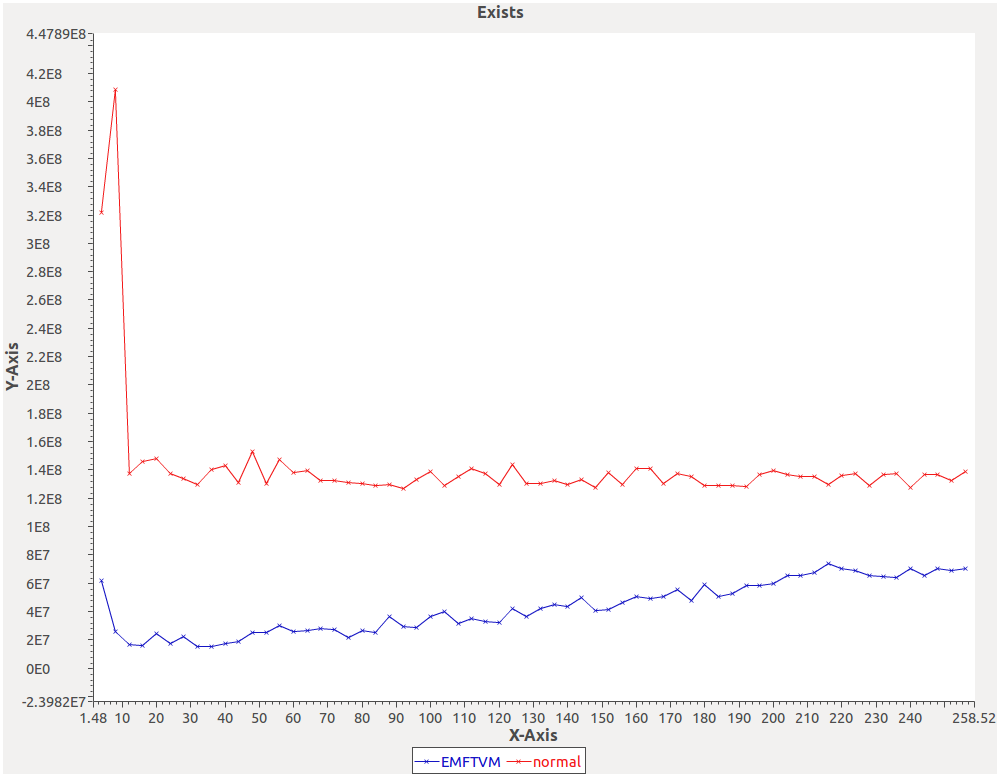
\includegraphics[width=\textwidth]{../graphs/sequence/Exists}
\end{figure*}
\pagebreak

\noindent\textbf{First}
\lstinputlisting[firstline=1,lastline=3]{../transformations/sequence/emftvm/TestFirst.atl}
\begin{figure*}[h]
\centering
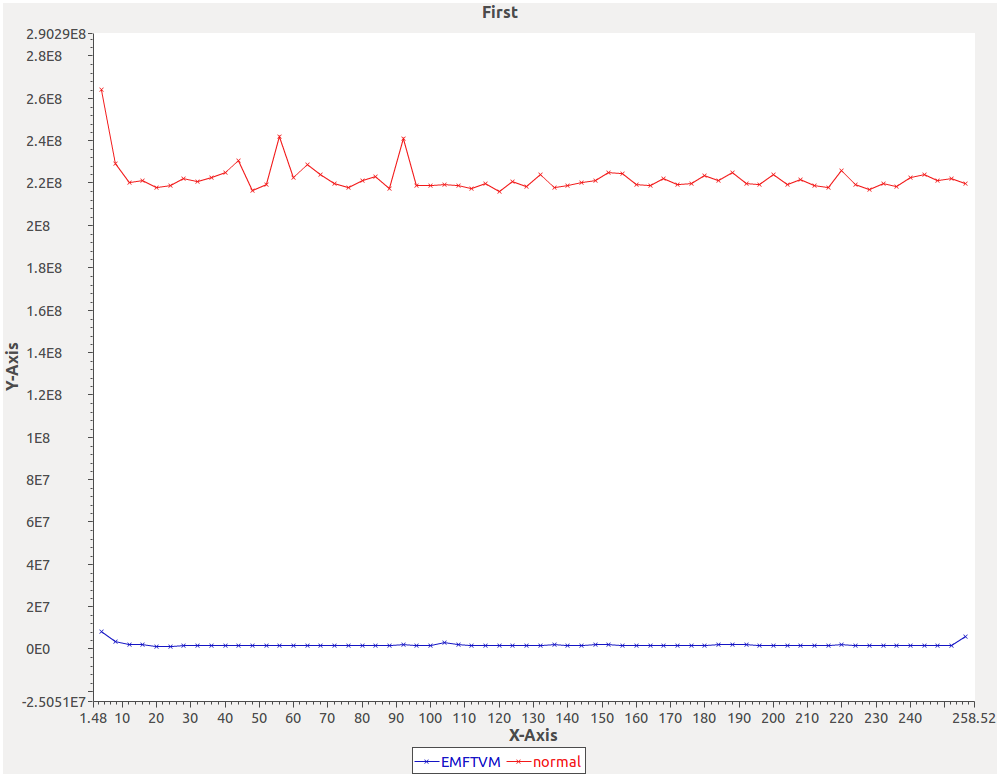
\includegraphics[width=\textwidth]{../graphs/sequence/First}
\end{figure*}
\pagebreak

\noindent\textbf{Flatten}
\lstinputlisting[firstline=1,lastline=3]{../transformations/sequence/emftvm/TestFlatten.atl}
\begin{figure*}[h]
\centering
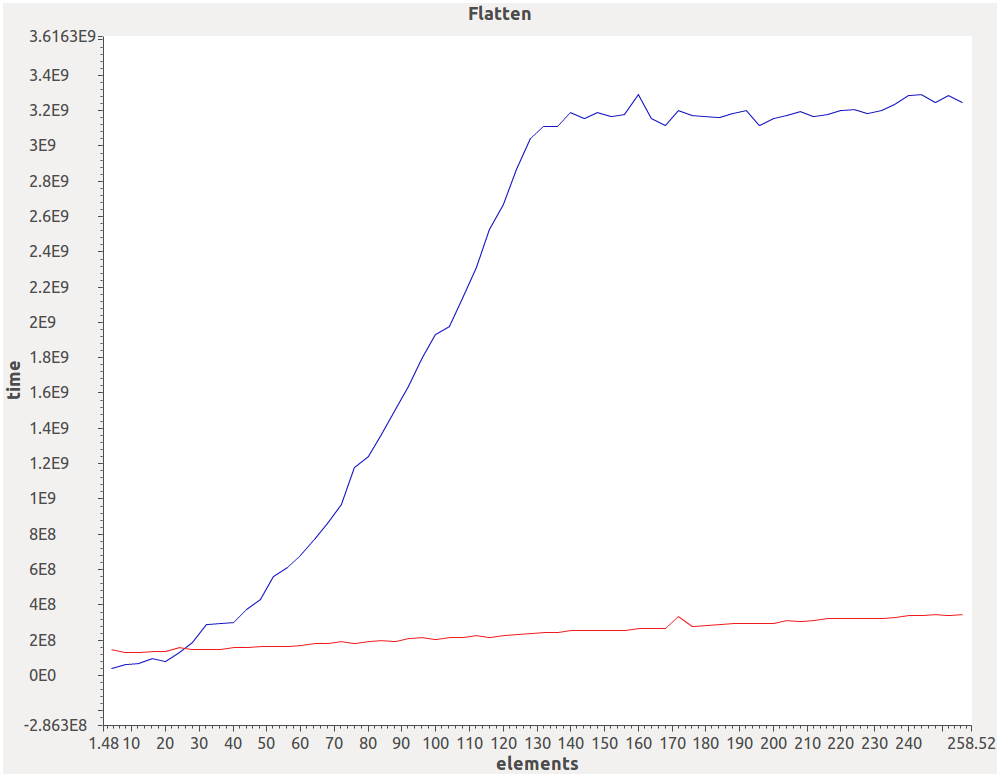
\includegraphics[width=\textwidth]{../graphs/sequence/Flatten}
\end{figure*}
\pagebreak

\noindent\textbf{ForAll}
\lstinputlisting[firstline=1,lastline=3]{../transformations/sequence/emftvm/TestForAll.atl}
\begin{figure*}[h]
\centering
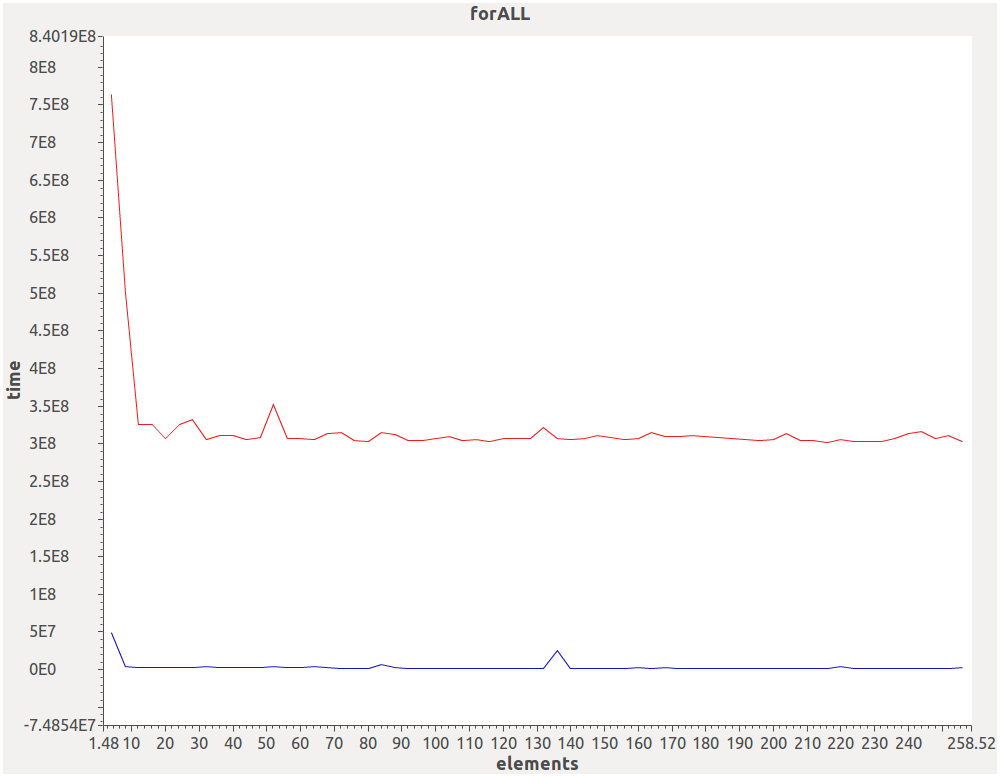
\includegraphics[width=\textwidth]{../graphs/sequence/forALL}
\end{figure*}
\pagebreak

\noindent\textbf{Includes}
\lstinputlisting[firstline=1,lastline=3]{../transformations/sequence/emftvm/TestIncludes.atl}
\begin{figure*}[h]
\centering
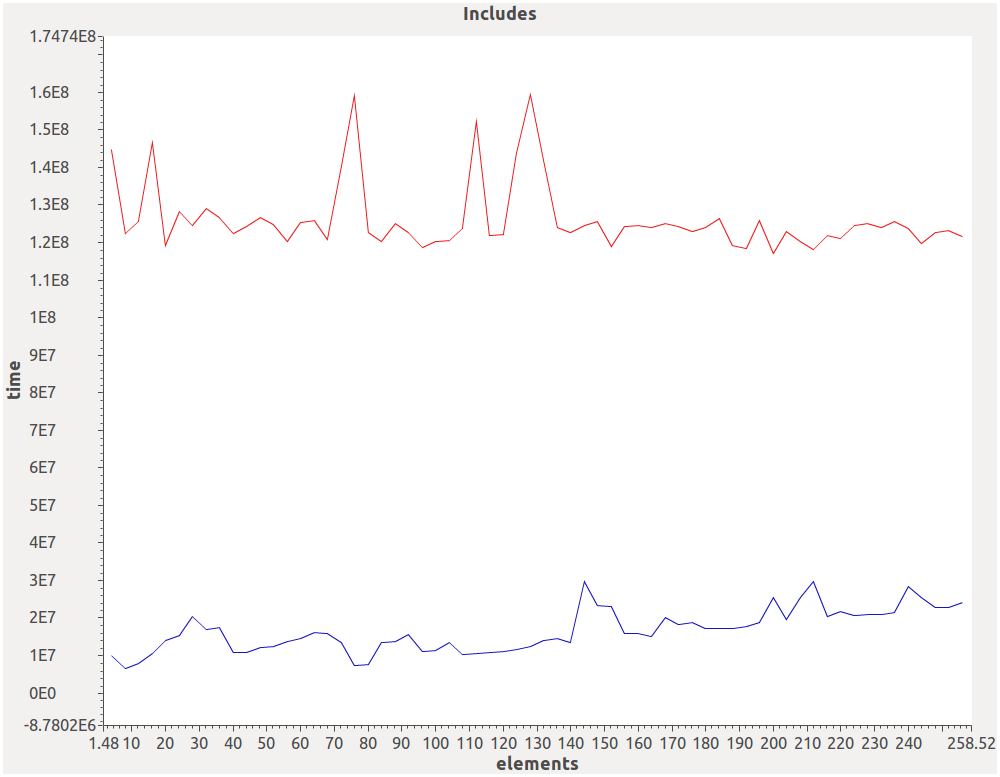
\includegraphics[width=\textwidth]{../graphs/sequence/Includes}
\end{figure*}
\pagebreak

\noindent\textbf{IncludesAll}
\lstinputlisting[firstline=1,lastline=3]{../transformations/sequence/emftvm/TestIncludesAll.atl}
\begin{figure*}[h]
\centering
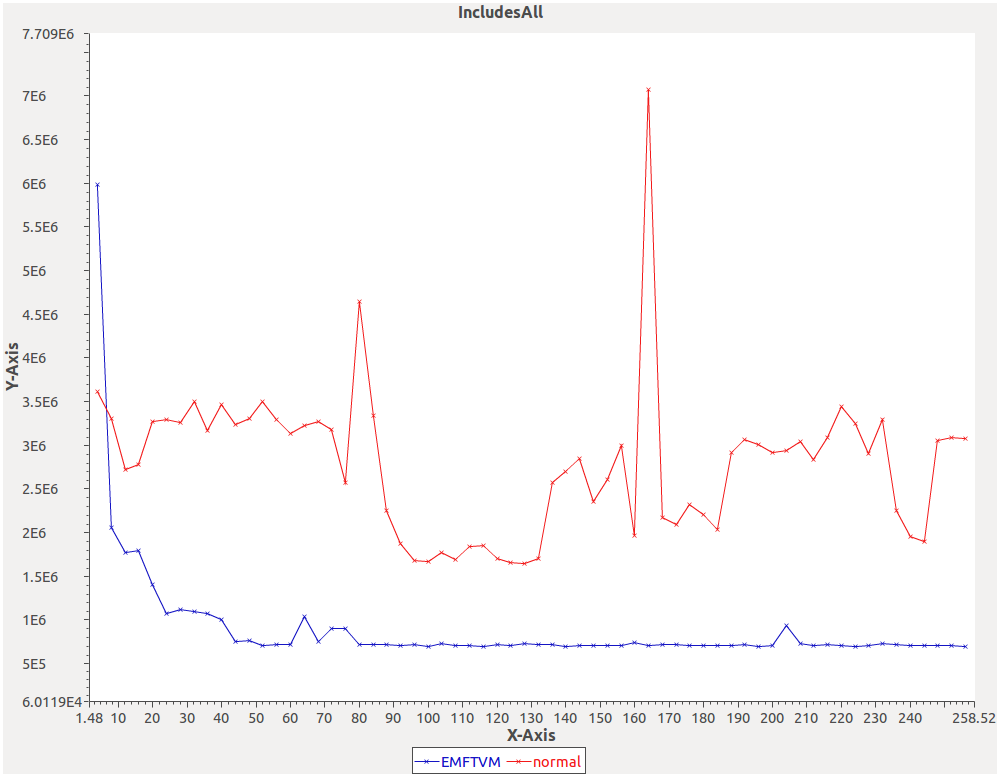
\includegraphics[width=\textwidth]{../graphs/sequence/IncludesAll}
\end{figure*}
\pagebreak

\noindent\textbf{Including}
\lstinputlisting[firstline=1,lastline=3]{../transformations/sequence/emftvm/TestIncluding.atl}
\begin{figure*}[h]
\centering
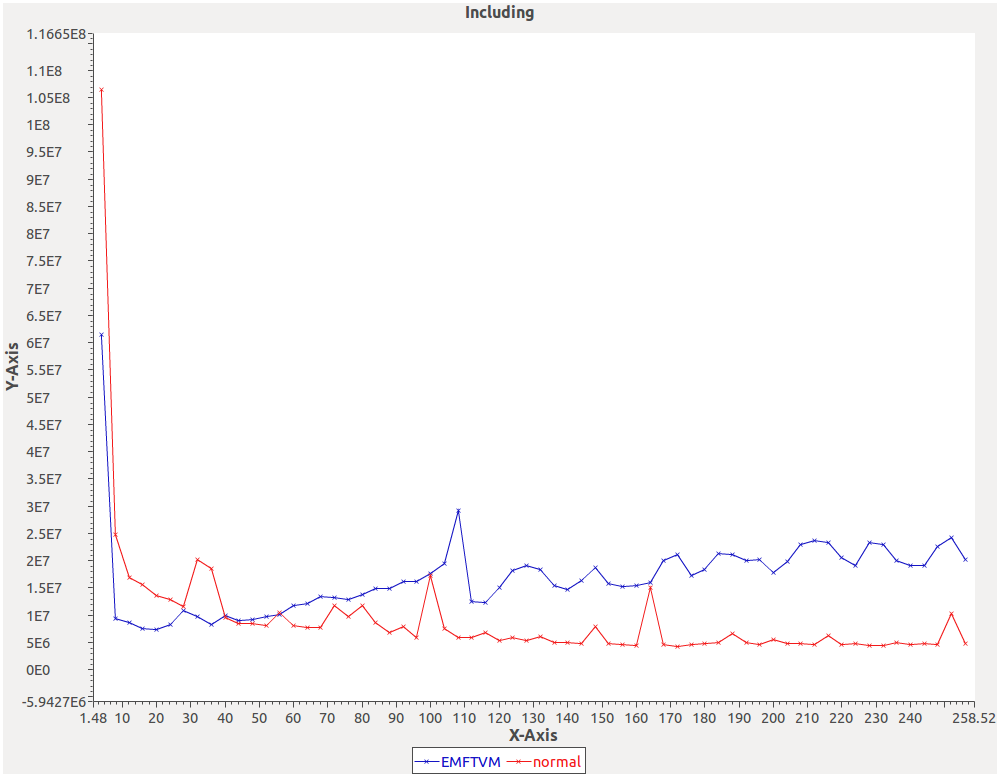
\includegraphics[width=\textwidth]{../graphs/sequence/Including}
\end{figure*}
\pagebreak

\noindent\textbf{IndexOf}
\lstinputlisting[firstline=1,lastline=3]{../transformations/sequence/emftvm/TestIndexOf.atl}
\begin{figure*}[h]
\centering
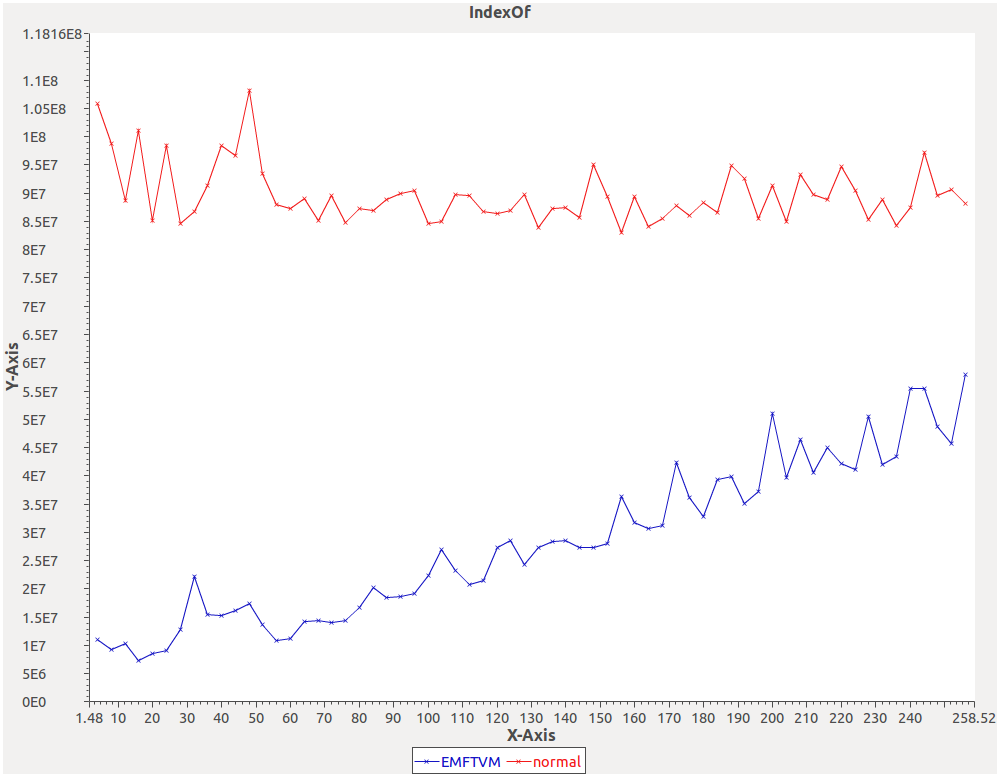
\includegraphics[width=\textwidth]{../graphs/sequence/IndexOf}
\end{figure*}
\pagebreak

\noindent\textbf{InsertAt}
\lstinputlisting[firstline=1,lastline=3]{../transformations/sequence/emftvm/TestInsertAt.atl}
\begin{figure*}[h]
\centering
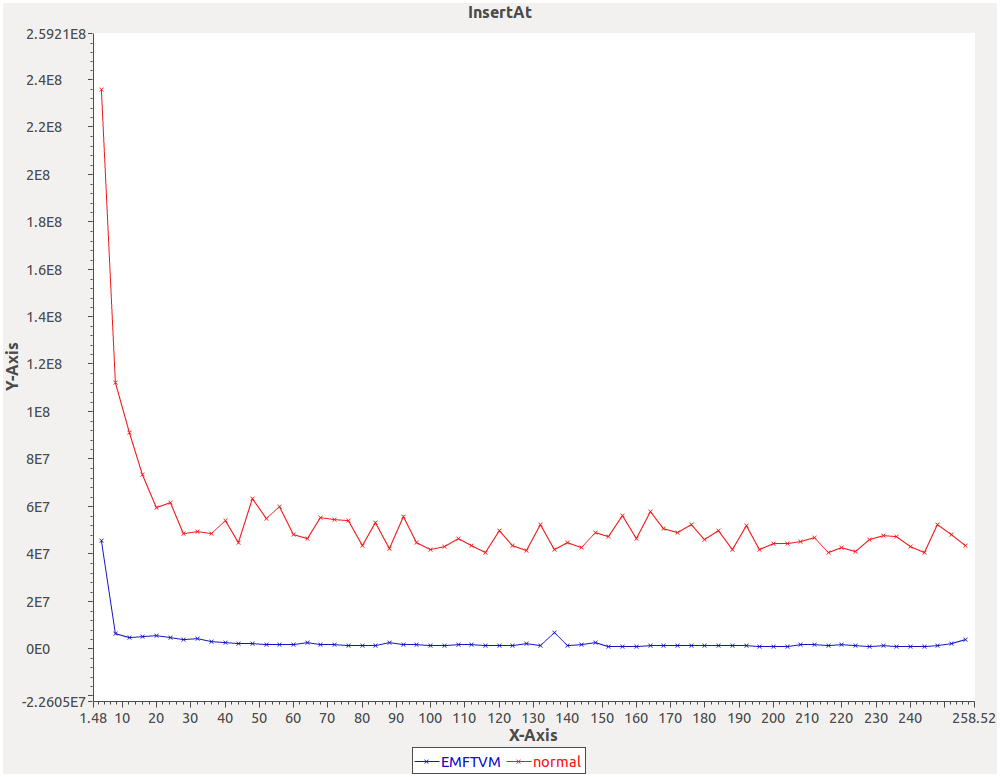
\includegraphics[width=\textwidth]{../graphs/sequence/InsertAt}
\end{figure*}
\pagebreak

\noindent\textbf{IsEmpty}
\lstinputlisting[firstline=1,lastline=3]{../transformations/sequence/emftvm/TestIsEmpty.atl}
\begin{figure*}[h]
\centering
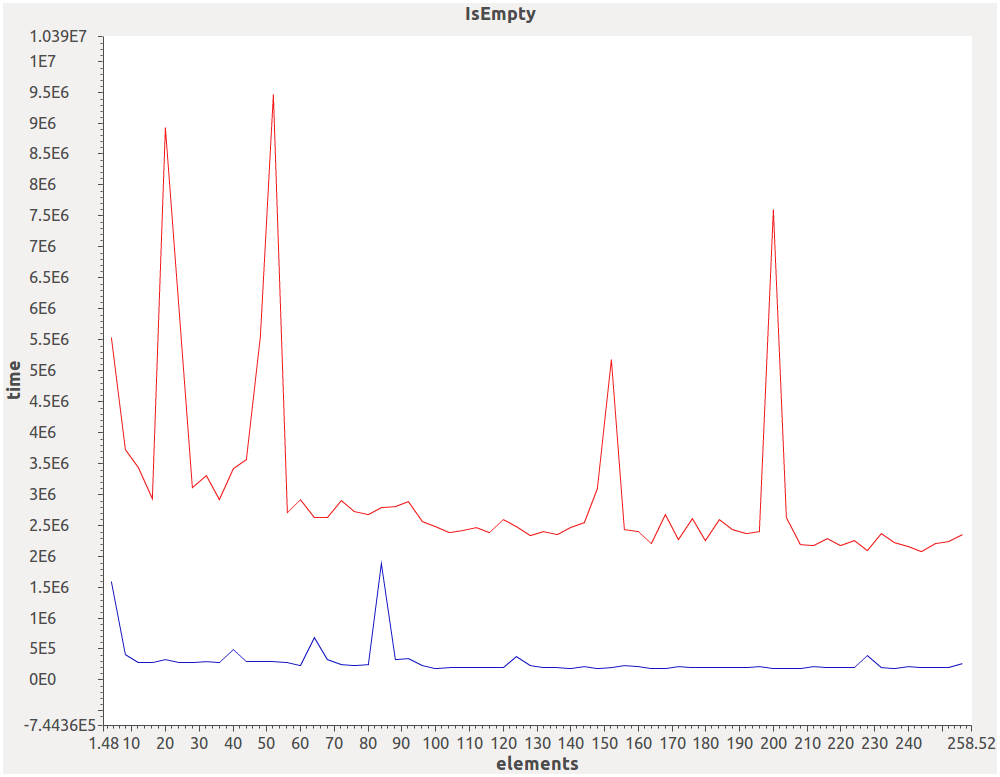
\includegraphics[width=\textwidth]{../graphs/sequence/IsEmpty}
\end{figure*}
\pagebreak

\noindent\textbf{IsUnique}
\lstinputlisting[firstline=1,lastline=3]{../transformations/sequence/emftvm/TestIsUnique.atl}
\begin{figure*}[h]
\centering
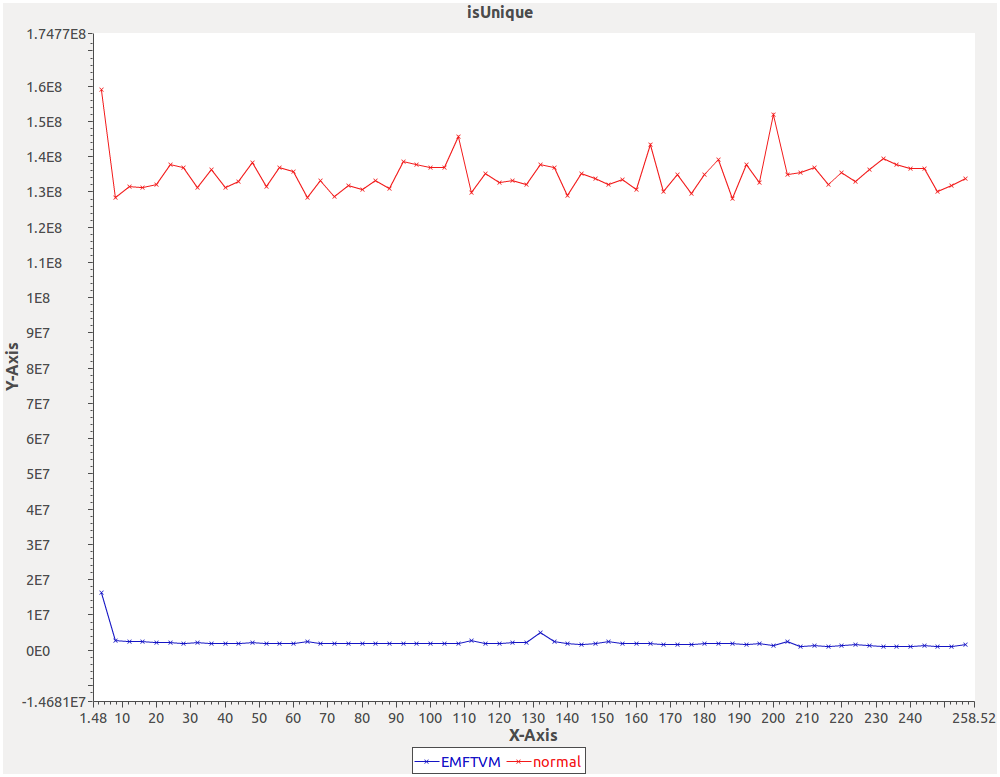
\includegraphics[width=\textwidth]{../graphs/sequence/isUnique}
\end{figure*}
\pagebreak

\noindent\textbf{Iterate}
\lstinputlisting[firstline=1,lastline=3]{../transformations/sequence/emftvm/TestIterate.atl}
\begin{figure*}[h]
\centering
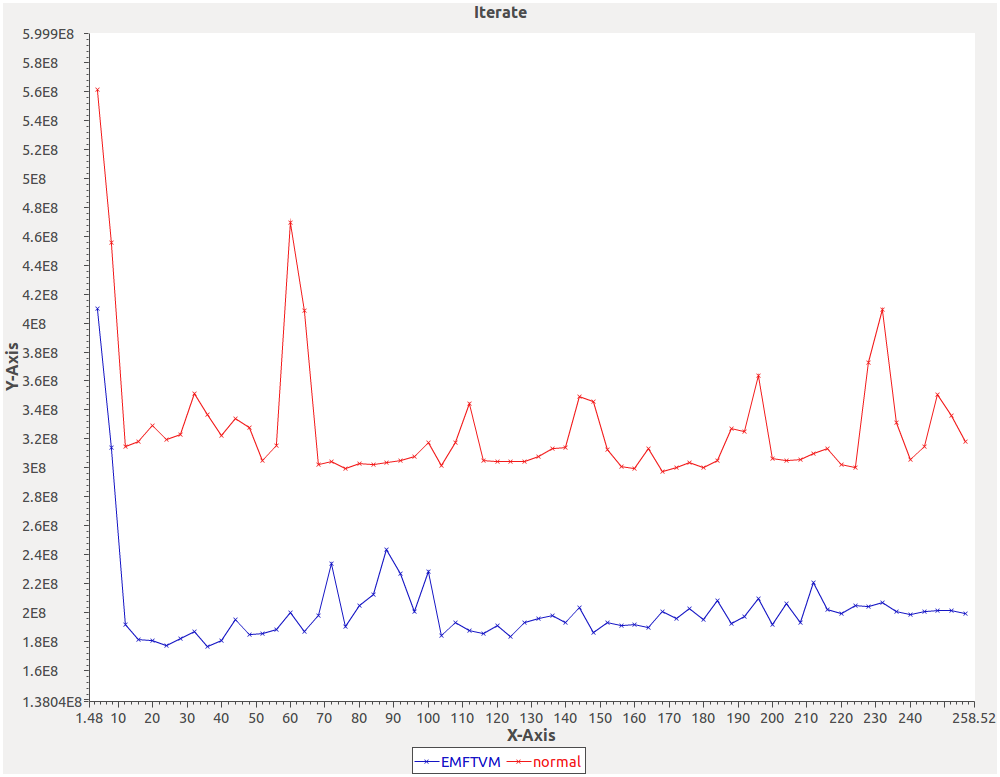
\includegraphics[width=\textwidth]{../graphs/sequence/Iterate}
\end{figure*}
\pagebreak

\noindent\textbf{Last}
\lstinputlisting[firstline=1,lastline=3]{../transformations/sequence/emftvm/TestLast.atl}
\begin{figure*}[h]
\centering
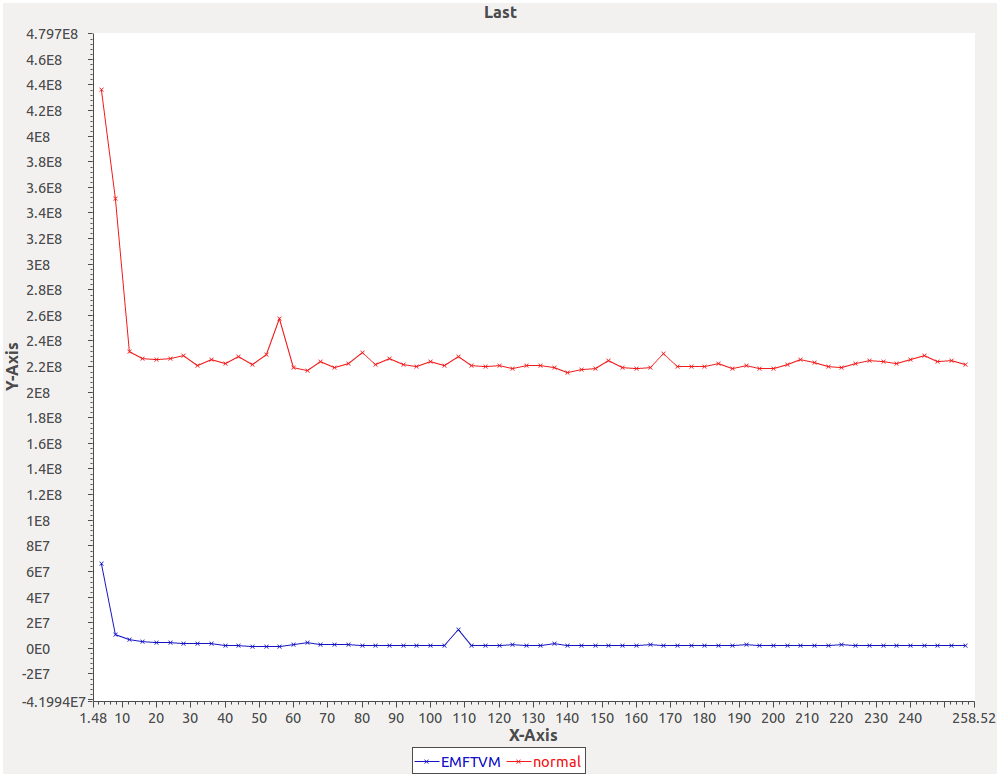
\includegraphics[width=\textwidth]{../graphs/sequence/Last}
\end{figure*}
\pagebreak

\noindent\textbf{NotEqual}
\lstinputlisting[firstline=1,lastline=3]{../transformations/sequence/emftvm/TestNeq.atl}
\begin{figure*}[h]
\centering
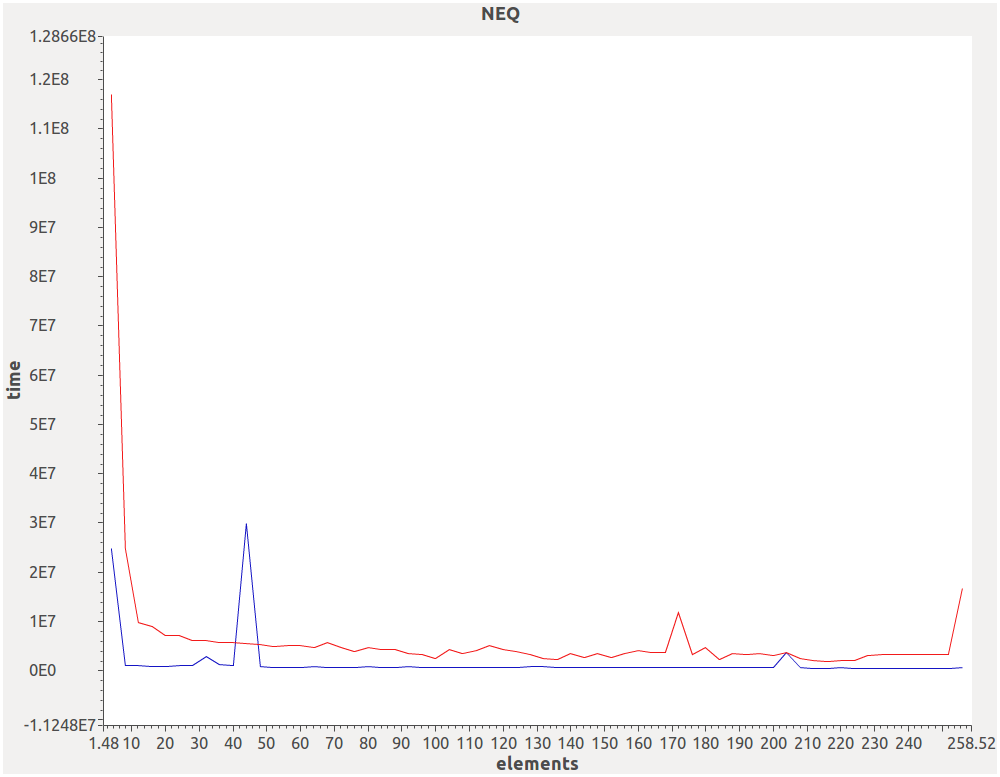
\includegraphics[width=\textwidth]{../graphs/sequence/NEQ}
\end{figure*}
\pagebreak

\noindent\textbf{One}
\lstinputlisting[firstline=1,lastline=3]{../transformations/sequence/emftvm/TestOne.atl}
\begin{figure*}[h]
\centering
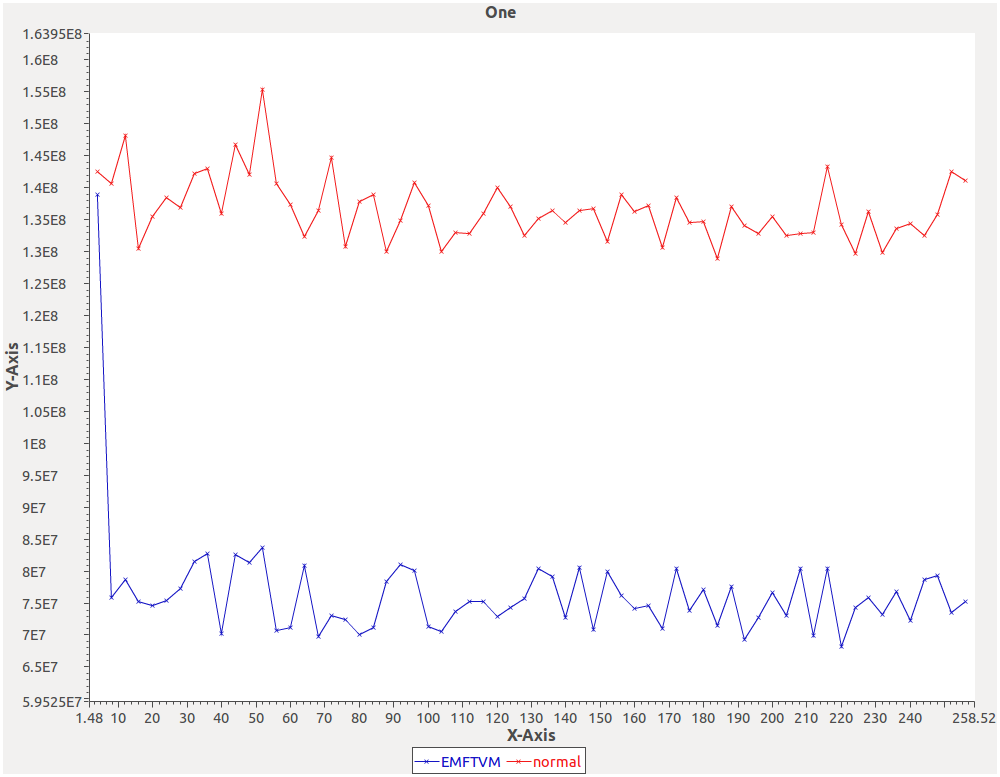
\includegraphics[width=\textwidth]{../graphs/sequence/One}
\end{figure*}
\pagebreak

\noindent\textbf{Prepend}
\lstinputlisting[firstline=1,lastline=3]{../transformations/sequence/emftvm/TestPrepend.atl}
\begin{figure*}[h]
\centering
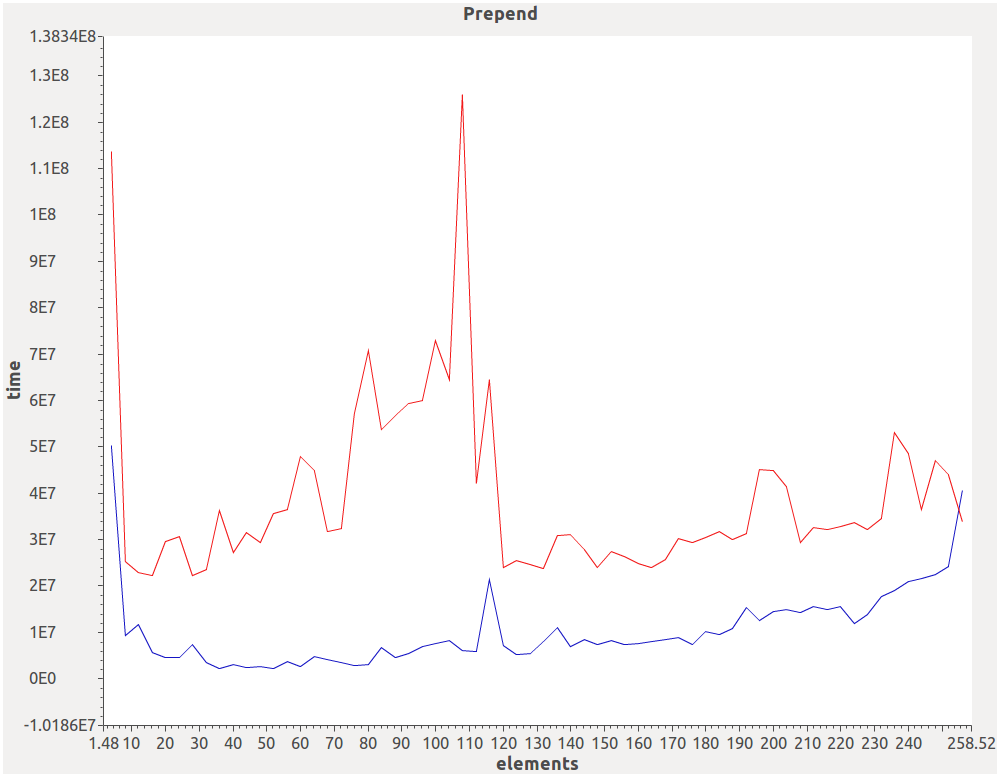
\includegraphics[width=\textwidth]{../graphs/sequence/Prepend}
\end{figure*}
\pagebreak

\noindent\textbf{Reject}
\lstinputlisting[firstline=1,lastline=3]{../transformations/sequence/emftvm/TestReject.atl}
\begin{figure*}[h]
\centering
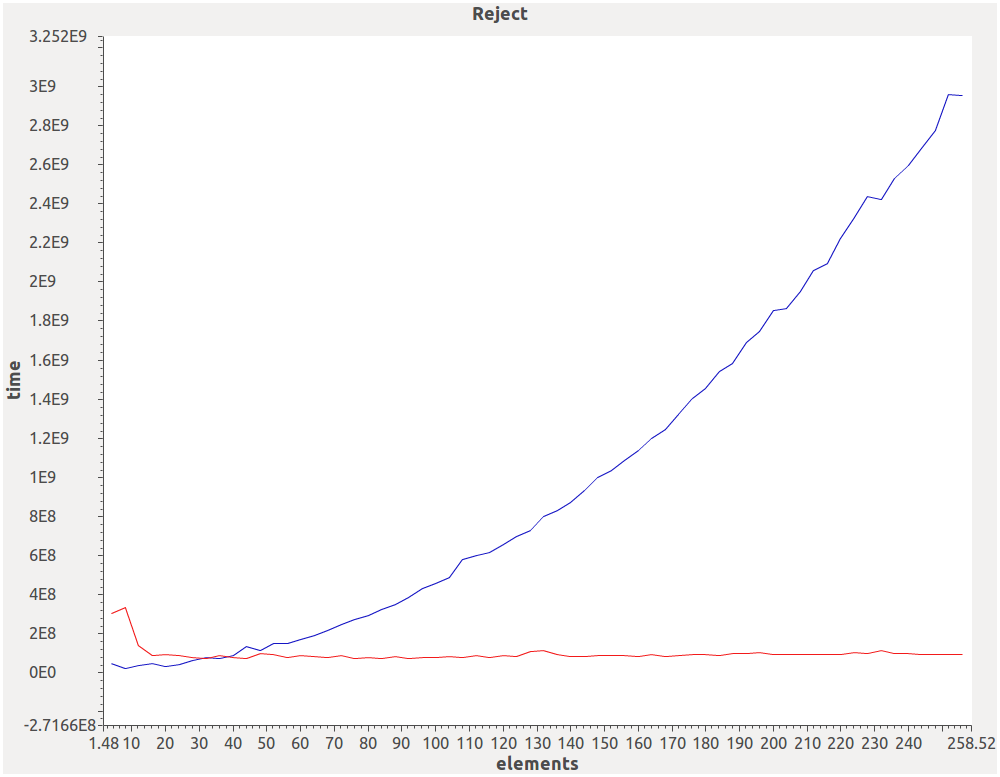
\includegraphics[width=\textwidth]{../graphs/sequence/Reject}
\end{figure*}
\pagebreak

\noindent\textbf{Select}
\lstinputlisting[firstline=1,lastline=3]{../transformations/sequence/emftvm/TestSelect.atl}
\begin{figure*}[h]
\centering
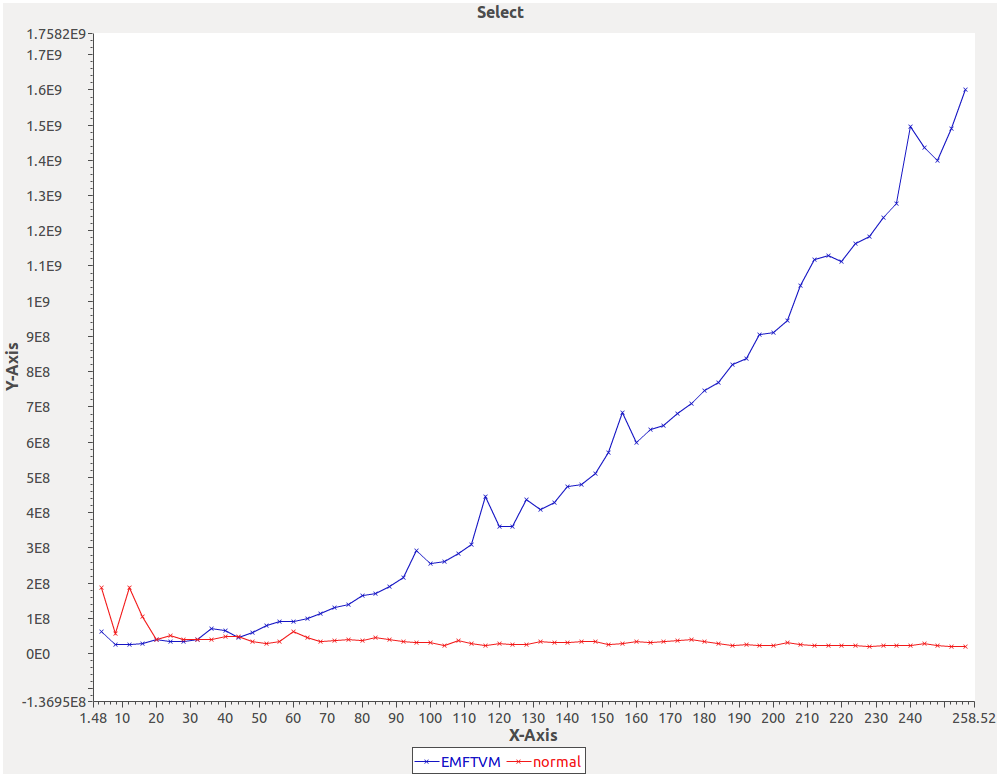
\includegraphics[width=\textwidth]{../graphs/sequence/Select}
\end{figure*}
\pagebreak

\noindent\textbf{Size}
\lstinputlisting[firstline=1,lastline=3]{../transformations/sequence/emftvm/TestSize.atl}
\begin{figure*}[h]
\centering
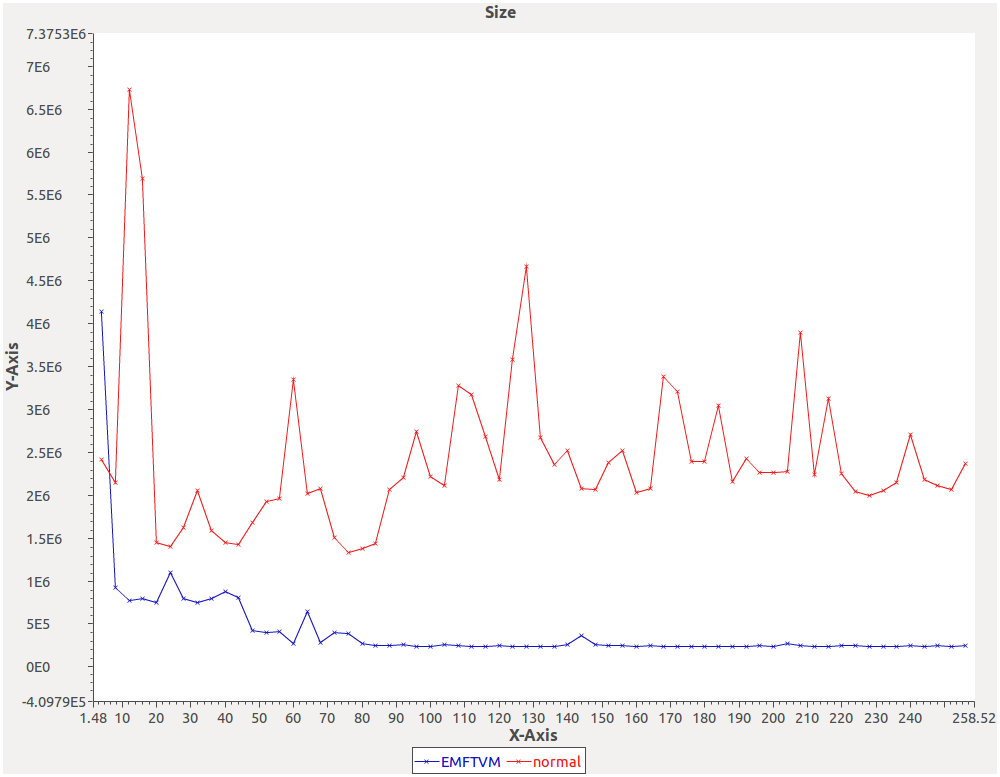
\includegraphics[width=\textwidth]{../graphs/sequence/Size}
\end{figure*}
\pagebreak

\noindent\textbf{SortedBy}
\lstinputlisting[firstline=1,lastline=3]{../transformations/sequence/emftvm/TestSortedBy.atl}
\begin{figure*}[h]
\centering
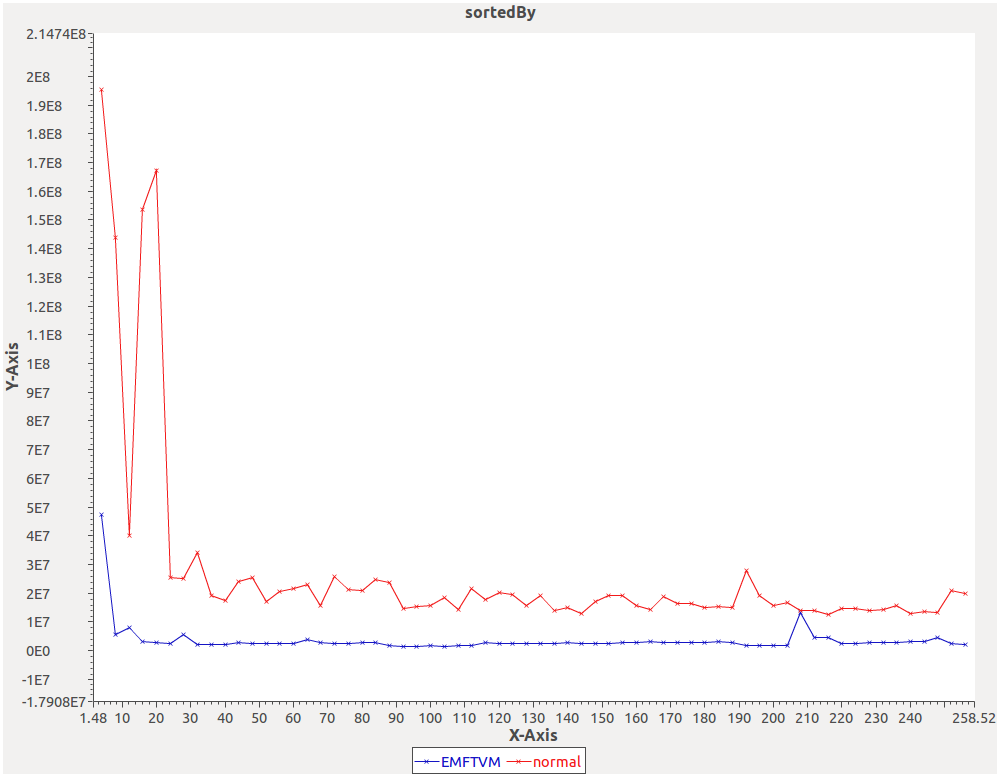
\includegraphics[width=\textwidth]{../graphs/sequence/sortedBy}
\end{figure*}
\pagebreak

\noindent\textbf{SubSequence}
\lstinputlisting[firstline=1,lastline=3]{../transformations/sequence/emftvm/TestSubsequence.atl}
\begin{figure*}[h]
\centering
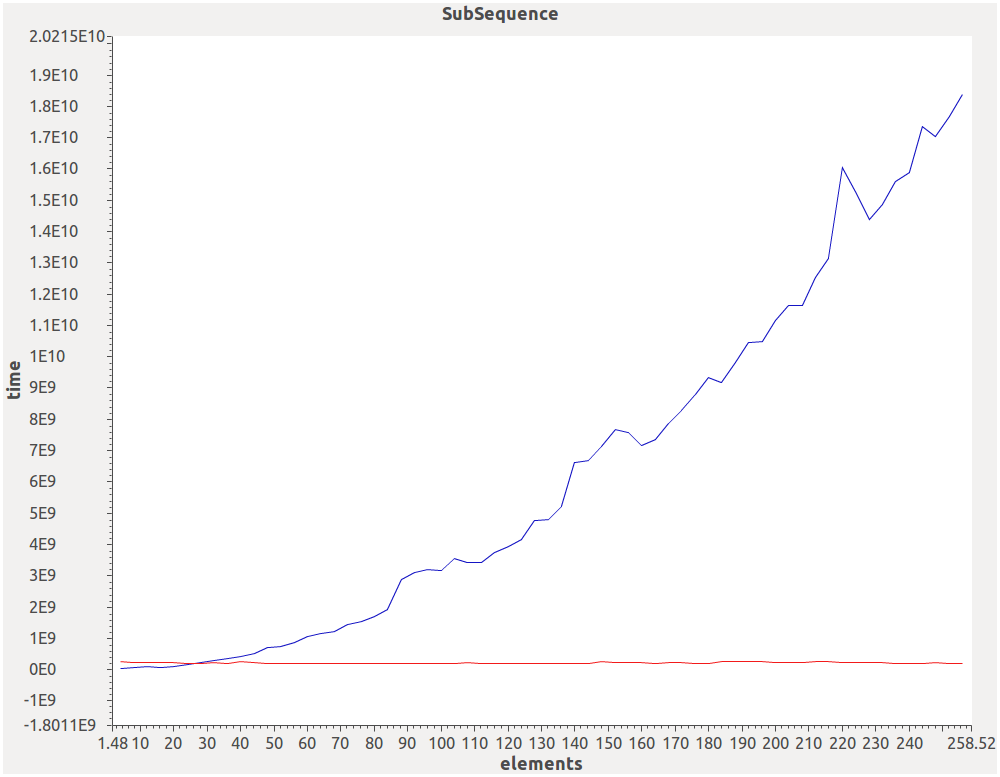
\includegraphics[width=\textwidth]{../graphs/sequence/SubSequence}
\end{figure*}
\pagebreak

\noindent\textbf{Sum}
\lstinputlisting[firstline=1,lastline=3]{../transformations/sequence/emftvm/TestSum.atl}
\begin{figure*}[h]
\centering
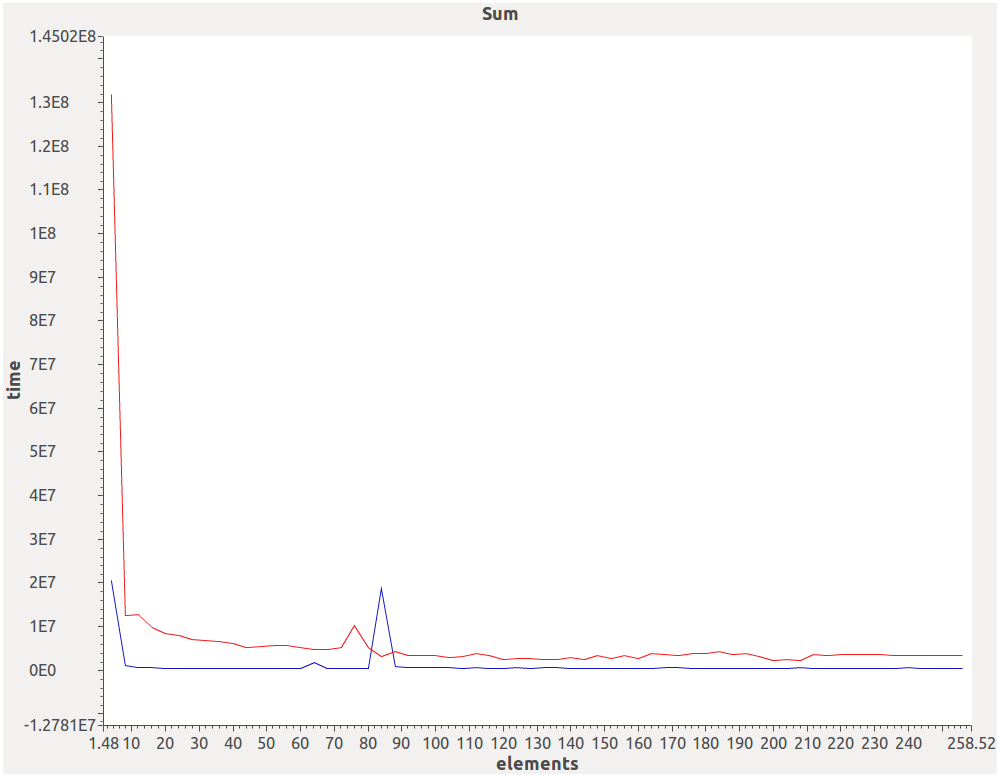
\includegraphics[width=\textwidth]{../graphs/sequence/Sum}
\end{figure*}
\pagebreak

\noindent\textbf{Union}
\lstinputlisting[firstline=1,lastline=3]{../transformations/sequence/emftvm/TestUnion.atl}
\begin{figure*}[h]
\centering
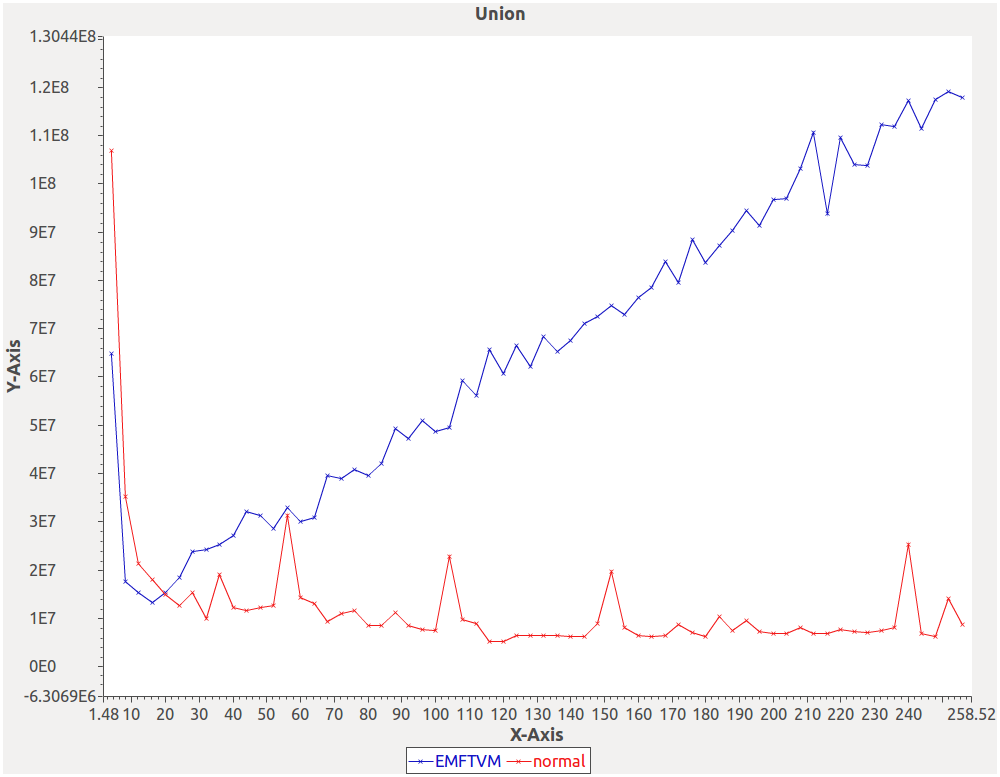
\includegraphics[width=\textwidth]{../graphs/sequence/Union}
\end{figure*}
\pagebreak